\chapter{Implementation}
\section{JBotSim: a Tool for Fast Prototyping of Distributed Algorithms in Dynamic Networks}
\paragraph{What's JBotSim ?}JBotSim is an open source simulation library that is dedicated to distributed algorithms in dynamic networks. It was developed with the purpose in mind to make it possible to implement an algorithmic idea in minutes and interact with it while it is running (e.g., add, move, or delete nodes). Besides interaction, JBotSim can also be used to prepare live demos of an algorithm and to show it to colleagues or students, as well as to assess the algorithm performance. JBotSim is not a competitor of mainstream simulators such as NS3 \cite{35}, OMNet \cite{40}, or The One \cite{38}, in the sense that it does not aim to implement real-world networking protocols. Quite the opposite, JBotSim aims to remain technology-insensitive and to be used at the algorithmic level, in a way closer in spirit to the ViSiDiA project (a general-purpose platform for distributed algorithms). Unlike ViSiDiA, however, JBotSim natively supports mobility and dynamic networks (as well as wireless communication). Another major difference with the above tools is that it is a library rather than a software: its purpose is to be used in other programs, whether these programs are simple scenarios of full-fledged software. Finally, JBotSim is distributed under the terms of the LGPL licence, which makes it easily extensible by the community.
\paragraph{}Whether the algorithms are centralized or distributed, the natural way of programming in JBotSim is event-driven: algorithms are specified as subroutines to be executed when particular events occur (appearance or disappearance of a link, arrival of a message, clock pulse, etc.). Movements of the nodes can be controlled either by program or by means of live interaction with the mouse (adding, deleting, or moving nodes around with left-click, right-click, or drag and drop, respectively). These movements are typically performed while the algorithm is running, in order to visualize it or test its behavior in challenging configurations.
\paragraph{}We offer a broad view of JBotSim's main features and design traits. We start with preliminary information in Section 2 regarding installation and documentation. Section 3 reviews $JBOTSIM’s$ main components and specificities such as programming paradigms, clock scheduling, user interaction, or global architecture. Section 4 zooms on key features such as the exchange of messages between nodes, graph-level APIs, or the creation of online demos. Finally, we discuss in Section 5 some extensions of JBotSim, including TikZ exportation feature and edge-markovian dynamic graph generator. Besides its features, the main asset of JBotSim is its simplicity of use – an aim that is pursued at the cost of re-writing it several times from scratch (the API is now stable).
\paragraph{Practical Aspects}In this short section, we show how to install JBotSim and run it with a first basic example (this step is not required to keep reading the present document). We also provide links to online documentation and examples, for readers who would like to explore JBotSim's features beyond this document.
\subparagraph{Fetching JBOTSIM}The straightest (and safest) way to obtain JBotSim is to fetch the latest release, as a jar package on  JBotSim’s website [1]. One can also get the latest development version from SourceForge’s GIT repository and compile it as shown below, keeping in mind that online documentation refers to the official release rather than this version. Here is the command:
\newline
> git clone git://git.code.sf.net/p/jbotsim/git target
\newline
where target is the local directory in which to put JBotSim. From that directory, one can produce the JAR package using a simple make. After more than seven years of development, JBotSim is finally approaching version 1.0 (as of today, version 1.0-prealpha) and we think it is ready to be tested by the community.
\subparagraph{First steps}As a first program, one can copy the code from Listing 5.1 into a file named HelloWorld.java.
\newpage
\begin{lstlisting} [caption=HelloWorld with JBOTSIM,captionpos=b]
import jbotsim.Topology;
import jbotsim.ui.JViewer;
public class HelloWorld{
	public static void main(String[] args){
		new JViewer(new Topology());
	} 
}
\end{lstlisting}

How to use the JAR file and run the HelloWorld example:
\begin{itemize}
	\item If using IntelliJ, go to Project structure > Modules (select the module) > Dependencies > "+" and add jbotsim.jar.
	\item If using Eclipse, go to Project > Properties > Java build path > Librairies > Add external jar and add jbotsim.jar.
	\item From the terminal, the following commands can be used:
		\begin{itemize}
			\item javac -cp jbotsim.jar HelloWorld.java (compilation)
			\item java -cp jbotsim.jar HelloWorld (execution)
		\end{itemize}
\end{itemize}

\subparagraph{}By running the program, one should see an empty gray surface in which nodes can be added, moved, or deleted using the mouse.
\subparagraph{Sources of documentation}In this document, we provide a general overview of what JBotSim is and how it is designed. This is by no means a comprehensive programming manual. The reader who wants to explore further some features or develop complex programs with JBotSim is referred to the API documentation (see javadoc on the website). \subparagraph{}Examples can also be found on JBotSim's website, together with comments and explanations. These examples offer a good starting point to learn specific components of the API from an operational standpoint – the present document essentially focuses on concepts. Most of the online examples feature embedded videos. Finally, most of the examples in this document are also available on JBotSim's website. Feel free to check them when the code given here is incomplete (e.g. I often omit package imports and main() methods for conciseness).
\paragraph{Features and Architecture}This section provides an overview of JBotSim's key features and discusses the reason why some design choices were made. I review topics as varied as programming paradigms, clock scheduling, user interaction, and global architecture.

\subparagraph{Basic features of nodes and links} 
\begin{figure}[h!]
	\centering
	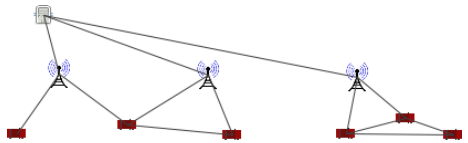
\includegraphics[width=0.7\linewidth]{fig_2}
	\caption[A highway scenario composed of vehicles, road-side units, and central servers. Part of the network is ad hoc (and wireless); the rest is infrastructured (and wired).]{A highway scenario composed of vehicles, road-side units, and central servers. Part of the network is ad hoc (and wireless); the rest is infrastructured (and wired).}
	\label{fig:fig2}
\end{figure}
\subparagraph{} JBotSim consists of a small number of classes, the most central being Node, Link, and Topology. The contexts in which dynamic networks apply are varied. In order to accommodate a majority of cases, these classes offer a number of conceptual variations around the notions of nodes and links. Nodes may or may not possess wireless communication capabilities, sensing abilities, or self-mobility. They may differ in clock frequency, color, communication range, or any other user-defined property. Links between the nodes account for potential communication among them. The nature of links varies as well; a link can be directed or undirected, as well as it can be wired or wireless – in the latter case  JBotSim's topology will update the set of links automatically, as a function of nodes distances and communication ranges.
\subparagraph{} JBotSim  consists of a small number of classes, the most central being Node, Link, and Topology. The contexts in which dynamic networks apply are varied. In order to accommodate a majority of cases, these classes offer a number of conceptual variations around the notions of nodes and links. Nodes may or may not possess wireless communication capabilities, sensing abilities, or self-mobility. They may differ in clock frequency, color, communication range, or any other user-defined property. Links between the nodes account for potential communication among them.
\newpage
The nature of links varies as well; a link can be directed or undirected, as well as it can be wired or wireless – in the latter case JBotSim's topology will update the set of links automatically, as a function of nodes distances and communication ranges.

Figure 5.2 illustrates a purely ad hoc scenario, whereby a heterogeneous swarm of UAVs and robots strives to clean a public park collectively. In this scenario, robots can detect and clean wastes of a certain type (red or blue) only if these are within their sensing range (depicted by a surrounding circle). However, they are pretty slow to move and cannot detect remote wastes. In the mean- time, a set of UAVs is patrolling over the park at higher speed and with larger sensing range. Whenever they detect a waste of some type, they store its position and start searching for a capable robot. In addition to sensing capabilities, UAVs can exchange messages with each other to optimize the process.
\subparagraph{}Besides nodes and links, the concept of topology is central in  JBotSim. Topologies can be thought of as containers for nodes and links, together with dedicated operations like updating wireless links. They also play a central role in  JBotSim's event architecture, as explained later on.
\begin{figure}[h!]
	\centering
	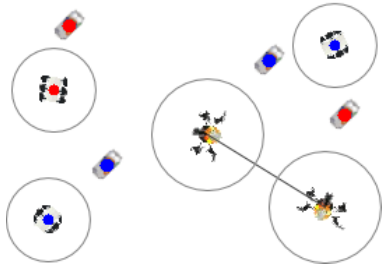
\includegraphics[width=0.5\linewidth]{fig_3}
	\caption[A swarming scenario, whereby mobiles robots and UAVs collaborate in order to clean a public park.]{A swarming scenario, whereby mobiles robots and UAVs collaborate in order to clean a public park.}
	\label{fig:fig3}
\end{figure}
\newpage
\subparagraph{Distributed vs. centralized algorithms}
\subparagraph{} JBotSim  supports the manipulation of centralized or distributed algorithms (possibly simultaneously). The natural way to implement a distributed algorithm is by extending the Node class, in which the desired behavior is implemented. Centralized algorithms are not constrained to a particular model, they can take the form of any standard java class.
\subparagraph{Distributed algorithm} JBotSim  comes with a default type of node that is implemented in the Node class. This class provides the most general features a node could have, including primitives for moving, exchanging messages, or tuning basic parameters (e.g. communication range and sensing range). Distributed algorithms are naturally implemented through adding specific features to this class. Listing 5.2 provides a basic example in which the nodes are endowed with self-mobility. The class relies on a key mechanism in  JBotSim : performing periodic operations that are triggered by the pulse of the system clock. This is done by overriding the onClock() method, which is called periodically by JBotSim’s engine (by default, at every pulse of the clock). The rest of the code is responsible for moving the node, setting a random direction at construction time (in radian), then moving in this direction periodically. (More details about the movement API can be found online.) Once this class is defined, new nodes of this type can be added to the topology in the same way as if they were of class Node, as illustrated in Listing 5.3. Here, a new topology is created first, then 10 nodes of the desired type (here, MovingNode) are added through the addNode() method at random locations (using $-1$ for $x$-coordinate or $y$-coordinate generates a random location for that coordinate; here both are random). In order to use MovingNode through the GUI, for instance when clicking with the mouse to add new nodes, this class must be registered as a node model. This is done by calling method setDefaultNodeModel() with the class itself as an argument, as shown on Listing 5.4. JBotSim will create new instances on the fly, using reflexivity. Several models can be registered simultaneously, using setNodeModel() with an additional argument that corresponds to the model name. If several models exist, JBotSim’s GUI (the viewer) displays a selection list when a node is added by the user (in this example, only one model is set and it is used by default). In the scenario of Figure 5.1, however, left-clicking on the surface would give the choice between car, tower, and server, the names of the three registered models for that scenario.
\begin{lstlisting} [caption=Extending the Node class,captionpos=b]
import jbotsim.Node;
public class MovingNode extends Node{
	public MovingNode(){
		setDirection(Math.random() * 2*Math.PI);
	}
	public void onClock(){
		move(2);
	}
}
\end{lstlisting}

\begin{lstlisting} [caption=Adding nodes manually,captionpos=b]
public static void main(String[] args){
	Topology tp = new Topology(400, 300);
	for (int i=0; i<10; i++)
		tp.addNode(-1,-1, new MovingNode());
	new JViewer(tp);
}
\end{lstlisting}

\begin{lstlisting}[caption=Using a defined node as default, captionpos=b]
public static void main(String[] args){
	Topology tp = new Topology(400, 300);
	tp.setDefaultNodeModel(MovingNode.class);
	new JViewer(tp);
}
\end{lstlisting}


\subparagraph{Centralized algorithms}There are many reasons why a centralized algorithm can be preferred over a distributed one. The object of study might be centralized in itself (e.g. network optimization, scheduling, graph algorithms in general). It may also be simpler to simulate distributed things in a centralized way. Listing 5.5 implements such a version of the random way-point mobility model, in which nodes repeatedly move toward a randomly selected destination, called target. Unlike a distributed implementation, the movements of nodes are here driven by a global loop at every pulse of the clock. For each node, a target is created if it does not exists yet or if it has just been reached; then the node’s direction is set accordingly and the node is moved (by default, by 1 unit of distance). For convenience, the main() method is included in the same class. Notice the use of setProperty() and getProperty() in this example. These methods allow to store any object directly into a node, using a key/value scheme (where key is a string). Both Link and Topology objects offer the same feature.
\begin{lstlisting}[caption=Example of a mobility trace recorder, captionpos=b]
public class CentralizedRWP implements ClockListener{
  Topology tp;
  public CentralizedRWP (Topology tp){
    this.tp = tp;
    tp.addClockListener(this);
  }
  public void onClock(){
    for (Node n : tp.getNodes()){
      Point2D target=(Point2D)n.getProperty("target");
      if (target == null || n.distance(target)<1){
        target = new Point2D.Double(Math.random()*400, Math.random()*300);
        n.setProperty("target", target);
        n.setDirection(target);
      }
      n.move();
    }
  }
  public static void main(String[] args){
    Topology tp = new Topology(400,300);
    new CentralizedRWP(tp);
    new JViewer(tp);
  }
}
\end{lstlisting}
\subparagraph{Architecture of the event system}
So far, we have seen one type of event: clock pulses, to be listened to through the ClockListener interface. JBotSim offers a number of such events and interfaces, some of which become are ubiquitous. The main ones are depicted on Figure 5.3 on the following page. This architecture allows one to specify dedicated operations in reaction to various events. For instance, one may ask to be notified whenever a link appears or disappears somewhere. Same for messages, which are typically listened to by the nodes themselves or can be watched at a global scale (e.g. to keep a log of all communications). In fact, every node is automatically notified for its own events; it just needs to override the corresponding methods from the parent class Node in order to specify event handlings (e.g. onClock(), onMessage(), onLinkAdded(), onSensingIn(), onSelection(), etc.). Explicit listeners, on the other hand, like the ones in Figure 5.3, are meant to be used by centralized programs which do not extend class Node. Listing 5.6 gives one such example, consisting of a mobility trace recorder. This program listens to topological events of various kinds, including appearance or disappearance of nodes or links, and movements of the nodes. Upon each of these events, it outputs a string representation of the event using a dedicated human readable format called DGS [7]. Similar code could be written for Gephi [3]. Other events exist besides those represented in Figure 5.3, such as the SelectionListener interface, which makes it possible to be notified when a node is selected (middle-click) and make it initiate some tasks, for instance broadcast, distinguished role, etc.
\subparagraph{Single threading: why and how?}It seems convenient at first, to assign every node a dedicated thread, however JBotSim was designed differently. JBotSim is single-threaded, and definitely so. This section explains the why and the how. Understanding these aspects are instrumental in developing well-organized and bug-free programs.
\begin{figure}[h!]
	\centering
	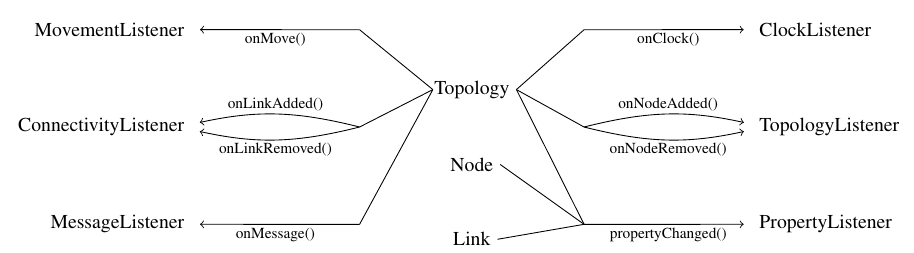
\includegraphics[width=1\linewidth]{fig_4}
	\caption[Main sources of events and corresponding interfaces in  JBotSim .]{Main sources of events and corresponding interfaces in  JBotSim .}
	\label{fig:fig4}
\end{figure}
\newpage
\begin{lstlisting}[caption=Example of a mobility trace recorder, captionpos=b]
public class MyRecorder implements TopologyListener, ConnectivityListener, MovementListener{
	public MyRecorder(Topology tp){
		tp.addTopologyListener(this);
		tp.addConnectivityListener(this);
		tp.addMovementListener(this);
	}
	// TopologyListener
	public void onNodeAdded(Node node) {
	 	println("an " + node.hashCode() +
	 		" x:" + node.getX() + " y:" + node.getY());
	 }
	 
	 public void onNodeRemoved(Node node) {
	 	println("dn " + node.hashCode());
	 }
	 // ConnectivityListener
	 public void onLinkAdded(Link link) {
	 	println("ae " + link.hashCode() + " " +
	 		link.endpoint(0) + " " + link.endpoint(1));
	 }
	 public void onLinkRemoved(Link link) {
	 	println("de " + link.hashCode());
	 }
	 // MovementListener
	 public void onNodeMoved(Node node) {
	 	println("cn " + node.hashCode() +
	 		" x:" + node.getX() + " y:" + node.getY());
	 	}
	 }
\end{lstlisting}
\subparagraph{}In JBotSim, all the nodes, and in fact all of JBotSim’s life (GUI excepted) is articulated around a single thread, which is driven by the central clock. The clock pulses at regular interval (whose period can be tuned) and notifies its listeners in a specific order.  JBotSim’s internal engines, such as the message engine, are served first. Then come those nodes whose wait period has expired (remind that nodes can choose to register to the clock with different periods). These nodes are notified in a random order. Hence, if all nodes listen to the clock at a rate of 1 (the default value), they will all be notified in a random order in each round, which makes  JBotSim’s scheduler a non-deterministic 2-bounded fair scheduler. (Other policies will be available eventually.) A simplified version of the current scheduling process is depicted on Figure 5.4.
\subparagraph{}One consequence of single-threading is that all computations (GUI excepted) take place in a sequential order that makes it possible to use unsynchronized data structures and simpler code. This also improves the scalability of JBotSim when the number of nodes grows large. One can rely on other user-defined threads in the program, however one should be careful that these thread do not interfer with  JBotSim’s. The canonical example is when a scenario is set up by program from within the thread of the main() method. If the initialization makes extensive use of  JBotSim’s API from within that thread and the clock starts triggering events at the same time, then problems might occur (and a Concurrent ModificationException be raised). The easy way around is to pause the clock before executing these instructions and to resume it after (using the pause() and the resume() methods on the topology, respectively).
\begin{figure}[h!]
	\centering
	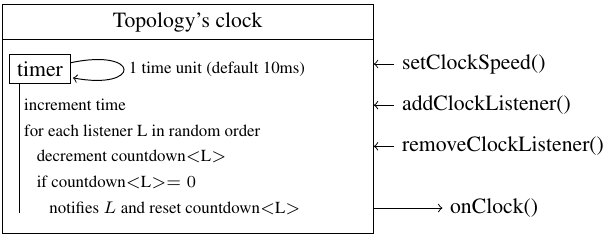
\includegraphics[width=.7\linewidth]{fig_5}
	\caption[Simplified version of the internal scheduler.]{Simplified version of the internal scheduler.}
	\label{fig:fig5}
\end{figure}
\subparagraph{Interactivity}JBotSim was designed with a clear separation in mind between GUI and internal features. In particular, it can be run without GUI (i.e. without creating the JViewer object), and things will work exactly the same, though invisibly. As such, JBotSim can be used to perform batch simulations (e.g. sequences of unattended runs that log the effects of some varying parameter). This also enables to withstand heavier simulations in terms of the number of nodes and links.
\subparagraph{}This being said, one of the most distinctive features of JBotSim remains interactivity, e.g., the ability to challenge the algorithm in difficult configurations through adding, removing, or moving nodes during the execution. This approach proves useful to think of a problem visually and intuitively. It also makes it possible to explain someone an algorithm through showing its behavior.
\subparagraph{}The architecture of  JBotSim’s viewer is depicted on Figure 5.5. As one can see, the viewer relies heavily on events related to nodes, links, and topology. The influence also goes the other way, with mouse actions being translated into topological operations. These features are realized by a class called JTopology. This class can often be ignored by the developer, which creates and manipulates the viewer through the higher JViewer class. The latter adds external features such as tuning slide bars, popup menus, or self-containment in a system window. 
\subparagraph{}While natural to  JBotSim’s users, the viewer remains, in all technical aspects, an independent piece of software. Alternative viewers could very well be designed with specific uses in mind.

\begin{figure}[h!]
	\centering
	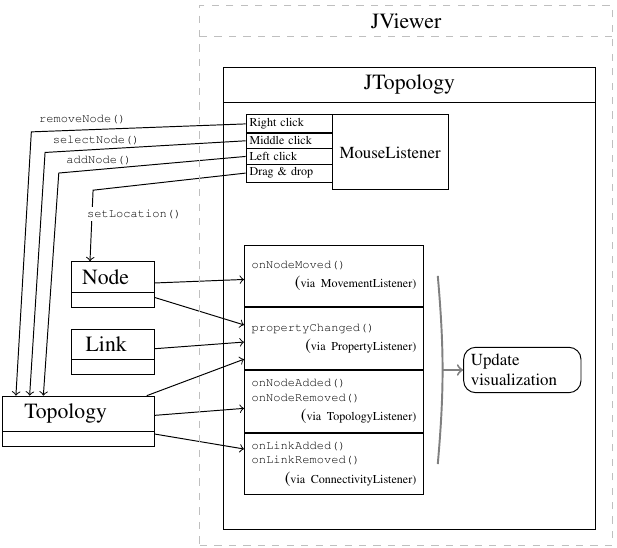
\includegraphics[width=.7\linewidth]{fig_6}
	\caption[Internals of JBotSim’s GUI]{Internals of JBotSim’s GUI}
	\label{fig:fig6}
\end{figure}
\paragraph{A zoom on selected features}This section provides more details on a handful of selected features. It covers, namely, the topics of message passing, graph-level algorithms, and java applets for online web demos.
\subparagraph{Exchanging messages}The way messages are used in JBotSim is independent from the communication technology considered. Indeed, the API is quite simple, messages are sent directly by the sender, through calling the send() method on its own instance (inherited from Node). Messages are typically received through overriding the onMessage() method (also from class Node). Another way to receive messages, which is not event-based, is for a node to check its mailbox manually through the getMailbox() method, for instance when it is executing the onClock() method (this is the natural way to implement round-based communication models). \subparagraph{}Listing 5.7 shows a message-based implementation of the flooding principle. Initially, none of the nodes are informed. Then, if a node is selected (either through middle-click or through direct call to the selectNode() method), then this node is notified in the onSelection() method and initiates a basic broadcast scheme. Here, the algorithm consists in retransmitting the received message upon first reception to all the local neighbors (sendAll()). In this example, the message is empty, however in general any object can be inserted in the message (no copy is made and the very same object is to be delivered, unless a copy is made at sending time). By default, a message takes one time unit to be transmitted (i.e. it is delivered at the next clock pulse). The delivery happens only for those links which exist by the time of reception. Since any object can be used as message content, it often has to be cast upon reception. All these aspects correspond to  JBotSim’s default message engine. Other message engines can be written, and indeed some exist in the jbotsimx package. For instance, the DelayMessageEngine makes it possible to add deterministic or random delays to the delivery of messages, possibly even in a non FIFO manner.
\newpage


\begin{lstlisting}[caption=Example of message passing algorithm, captionpos=b]
public class FloodingNode extends Node{
	boolean informed = false;
	@Override 
	public void onSelection() {
		informed = true;
		sendAll(new Message());
	}
	@Override
	public void onMessage(Message message) {
		if (!informed){
			informed = true;
			sendAll(message);
		}
	}
}
\end{lstlisting}
\subparagraph{Working at the graph level}Implementing an algorithm in the message passing model is sometimes difficult. JBotSim makes it possible to sketch an idea, play with it, and share it with others, in minutes, thanks to working at a (more abstract) graph-level. This level of abstraction also is relevant in its own right, when the object of study is itself at the graph level, such as classical graph algorithms or distributed coarse-grain models like graph relabeling systems [39] or population protocols [32].
\subparagraph{}To illustrate the simplicity of the graph level, let us consider a scenario where a type of node called SocialNode, dislikes being isolated. Such a node is happy (green) if it has at least one neighbor, unhappy (red) otherwise. In the message passing paradigm, this principle would require to send periodic messages (beacons) and track the reception of these messages, as well as using a timer to decide when a node becomes isolated. Listing 5.8 shows a possible implementation at the graph level, which is pretty concise and self-explanatory. Topological events are directly detected by the nodes, which can update their status. (These events could also be listened to globally through the ConnectivityListener() interface. This is the way one might want to implement centralized dynamic graph algorithms. Of course, from a message passing perspective, this implementation is cheating. Thus, methods like onLinkAdded(), hasNeighbors(), or getNeighbors() should not be used in a message-passing setting.

\begin{lstlisting}[caption=Example of graph-based algorithm, captionpos=b]
public class SocialNode extends Node{
	public SocialNode(){
		setColor(Color.red);
	}
	public void onLinkAdded(Link l){
		setColor(Color.green);
	}
	public void onLinkRemoved(Link l){
		if (!hasNeighbors())
			setColor(Color.red);
		}
	}
}
\end{lstlisting}
\subparagraph{Embedding JBOTSIM in a java applet}One of the features of  JBotSim’s viewer is to create a windowed frame automatically for the topology. This is the default behavior of JViewer’s constructor when a single parameter of type Topology or JTopology is used. Other behaviors can be obtained by using different versions of the constructor. In particular, one can specify that no windowed frame should be created, and the JTopology object be plugged manually into a different container. This feature enables the customization of JBotSim’s UI at will, as well as the creation of java applets.
\subparagraph{}Listing 5.9 shows an example java applet corresponding to the HelloWorld program from Listing 5.1. Here, a JTopology object (which is a JPanel) is created manually from the topology. Its reference is then used to augment it with standard viewer features, and finally added to the applet container. Another important step is to pause the clock in the destroy() method (otherwise JBotSim’s engine would keep running in background).
\newpage
\begin{lstlisting}[caption=Embedding a JBotSim demo into a java applet, captionpos=b]
import javax.swing.JApplet;
import jbotsim.Clock;
import jbotsim.Topology;
import jbotsim.ui.JTopology;
import jbotsim.ui.JViewer;
@SuppressWarnings("serial")
public class HelloWorld_Applet extends JApplet{
	Topology tp;
	public void init(){
		tp = new Topology();
		JTopology jtp = new JTopology(tp);
		new JViewer(jtp, false);
		this.add(jtp);
	}
	public void destroy(){
		tp.pause();
	}
}
\end{lstlisting}

\paragraph{Concluding remarks}We can say that JBotSim is a kernel, in the sense that it encapsulates a number of generic features whose purpose is to be used by higher programs. As of today, the plan is to keep it this way and try containing the growth of the number of features, to the profit of quality and simplicity. This does not mean, of course, that JBotSim should not be extended externally.
\paragraph{}In particular, JBotSim’s distribution already incorporates an extension package called jbotsimx, in which more specific features could be found. For instance, it incorporates a static class called Tikz that makes it possible to export the current topology as a TikZ picture – a powerful format for drawing pictures in LATEX documents. Figure 5.6 illustrates this with two pictures that have been generated. The Tikz class is composed of a single method, exportAsTikz(), which takes a mandatory Topology argument, and an optional scaling argument.
\paragraph{}Other extensions include basic topology algorithms for testing, e.g., if a given topology is connected or 2-connected, if a given node is critical (its removal would disconnect the graph) or compute the diameter. A set of extensions dedicated to dynamic graph are currently being developed (by others). For instance, the EMEGPlayer takes as input a birth rate, death rate, and an underlying graph (given as a Topology), and generates an edge-markovian dynamic graph based on these parameters, the dynamics of which can be listened to through the ConnectivityListener interface.

\begin{figure}[h]
	\centering
	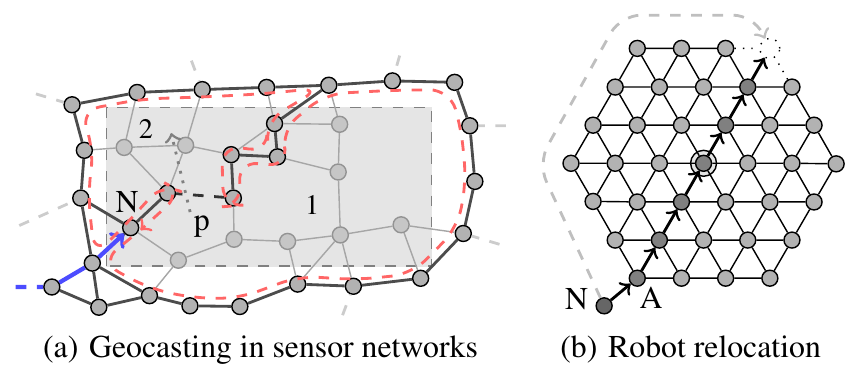
\includegraphics[width=0.7\linewidth]{fig_7}
	\caption[Two examples of pictures whose underlying topology was generated using JBotSim Tikz extension.]{Two examples of pictures whose underlying topology was generated using JBotSim Tikz extension. The topology on the left was created by adding and moving nodes using the mouse; the topology on the right was generated by program. Once exported as a Tikz picture, they were twicked manually to add shading, color, etc.}
	\label{fig:fig7}
\end{figure}

\begin{figure}
	\centering
	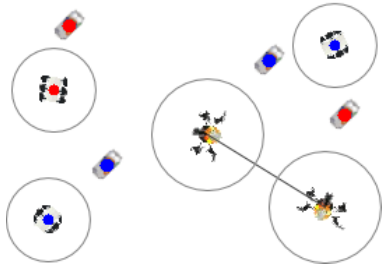
\includegraphics[width=0.7\linewidth]{fig_3}
	\caption[dgfs]{sdfsdfsdf}
	\label{fig:fig3}
\end{figure}



\section{Performance Analysis}

This section presents performance characteristics of our algorithm measured through simulations using JBotSim \cite{31} tool. We consider the following metrics defined for any component of size $n$.

\begin{enumerate}
	\item \textbf{Latency} $l$. The number of rounds necessary for a component to elect a leader (become stable) after a topology change (average over all initial topologies).
	
	\item \textbf{Sensitivity} $s$. The number of nodes that updated their heights in response to a topology change (average over all possible topology changes).
	
	\item \textbf{Resilience} $r$. The maximal fraction of links which can go down in a stable component without reelecting the current leader.
	
\end{enumerate}

We have measured these parameters using simulations of several scenarios (Figures 5.6(a) and 5.6(b)), and we summarize them below:

\begin{itemize}
	\item Merging two stable components:
	
	\begin{itemize}
		\item Given two fully connected (every two nodes are neighbours) components: $l \simeq 2$.
		\item Given two poorly connected (a node can have not more than two neighbours) components: $l \simeq n$.
	\end{itemize}
	
	\item Partitioning a stable component:
	
	\begin{itemize}
		\item Getting two fully connected component: $l = 2$.
		\item Getting two poorly connected component: $l = 2n$.
	\end{itemize}
	
	\item Topology change in a “small world-like” stable component (every node has $O(log~n)$ neighbours) without partitioning:
	\begin{itemize}
		\item Latency $l$ = $O(1)$.
		\item Sensitivity $s$ = $O(log(n))$.
	\end{itemize}
	
	\item Resilience of a stable component:
	
	\begin{itemize}
		\item Given a fully connected component: $r \approx 1 - 2/n$.
		\item Given a “small world-like” component: $r \approx 1 - 2/log(n)$.
	\end{itemize}
	
\end{itemize}


\begin{figure}[hbtp]
	\centering
	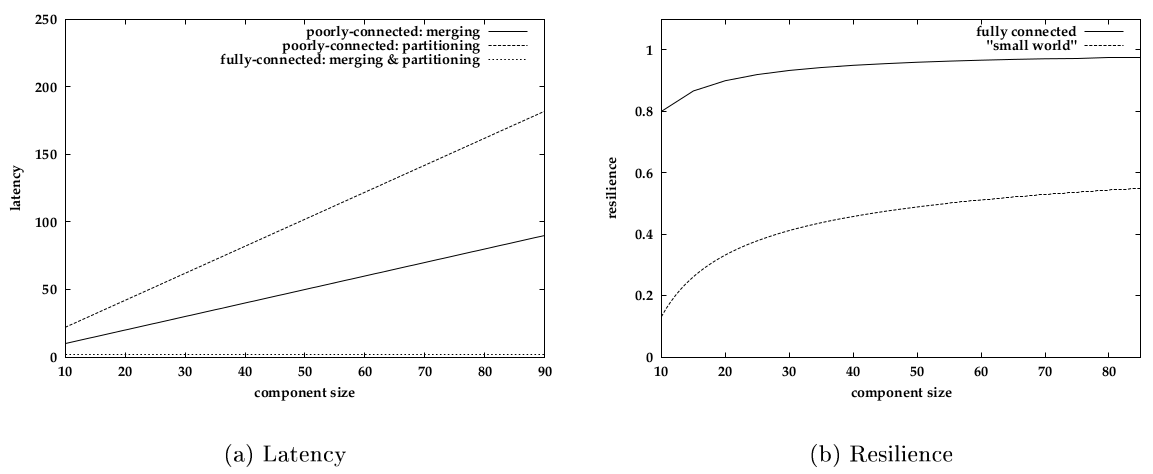
\includegraphics[scale=.4]{performance_test.png}
	\caption{Simulation results}
\end{figure}
